\section{Implementation Overview}
\sink\ is implemented entirely in Python using the PyCCN \cite{pyccn} wrapper around CCNx. Currently, all functionality except transport layer semantic translation is implemented. The design of \sink\ can be viewed from two perspective: the gateway component and the bridge component. Though the bridge component uses elements of the gateway to minimize redundant code, the designs of each are mostly independent. In this section we describe each of them in more detail. 

\subsection{Gateway Implementation}
The core design of the gateway can be perceived as the composition of two flexible pipelines that route traffic from NDN (resp. IP) networks to IP (resp. NDN) networks (see Figure \ref{fig:pipeline}). Each pipeline begins and ends with an {\tt InputStage} and {\tt OutputStage}, respectively, one for the IP network and one for the NDN network. Each {\tt InputStage} instance runs an appropriate interface to the network from which it receives traffic. Specifically, the {\tt IPInputStage} runs an HTTP server to intercept IP-to-NDN interests, and the {\tt NDNInputStage} registers a CCNx handle and configures an interest filter for incoming interests. 

\begin{figure*}[ht!]
\begin{center}
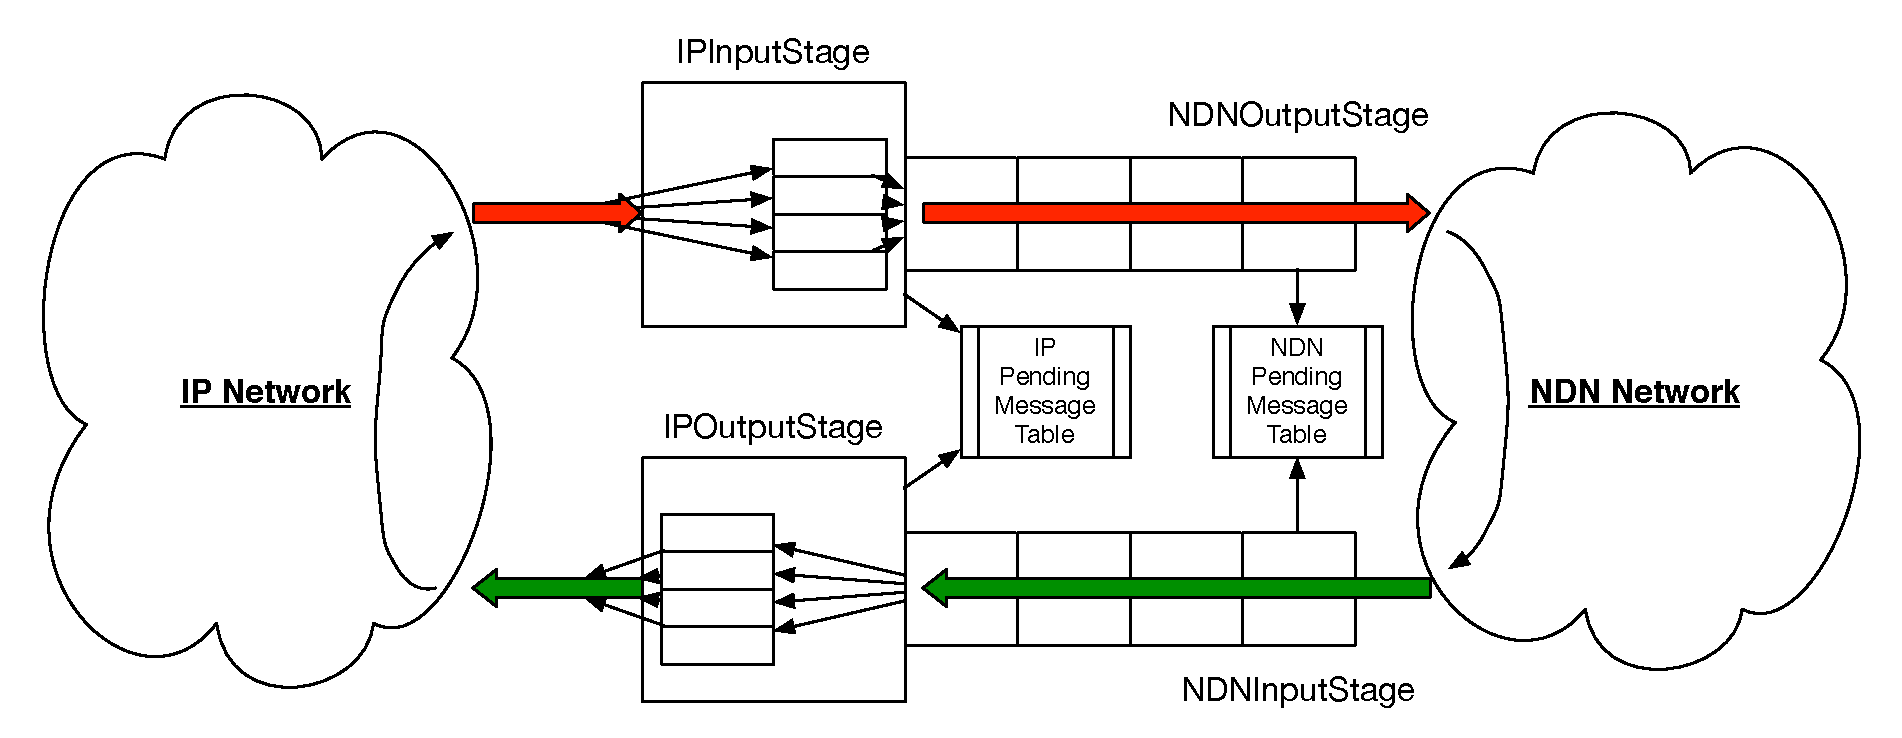
\includegraphics[scale=0.45]{./images/pipeline.pdf}
\label{fig:pipeline}
\caption{Bidirectional message pipeline for IP-to-NDN and NDN-to-IP message traversal.}
\end{center}
\end{figure*}

It is important to emphasize that the {\tt NDNInputStage} operates independently of the underlying network implementation. In a true deployment, CCNx would not be used to interface with the NDN network. Rather, a CCN network stack would be implemented on top of the appropriate network interface controller (NIC). The mechanism for registering an interest filter on top of this network stack would change, but the functionality that happens after an interest is intercepted will remain the same. Using CCnx for the preliminary development of this gateway was necessary since there does not yet exist NDN NICs or CCN software stacks that are not built upon the TCP/IP stack.

After an input stage receives an incoming message (i.e., an IP packet or NDN interest), the asynchronous message handler will (1) allocate an entry in the \emph{pending message table} for the network interface, (2) decompose the components of the message into its ``raw form'' and (3) save them in common message object wrapper, and (4) forward the resulting object to the next pipeline stage. For example, the {\tt IPInputStage} will save the IP source host and port information in the {\tt IPPendingMessageTable}, extract the URI path and set it as the ``destination'' field in the outgoing message object, and forward this message object to the next pipeline stage. In addition to the message source information for each entry in the pending message table, a binary semaphore is also stored. After forwarding the object, each handler will acquire a lock on this binary semaphore until the content associated with this message is retrieved from the target network. 

The pipeline is designed so that each stage (with the exception of the {\tt InputStage}) has a thread-safe input queue and a reference to the next stage (with the exception of the {\tt OutputStage}). This simple interface and design enables any number of intermediate stages to be configured between the input and output stages. For simplicity, the current \sink\ implementation only uses two stages - input and output stages. 

Once a message reaches the output stage, a new message for the target network is created and issued to the network. For example, an NDN interest will be formatted based on the contents of the outgoing message object retrieved from the output stage queue. After the target network returns content, the input stage of the target network performs the following tasks: First, the pending message table is checked for the an entry corresponding to the input message (e.g., an interest name that matches name of a previously issued interest). If an entry is found, the content field of the matching entry is populated and the binary semaphore associated with the semaphore is released. The latter step unblocks the original asynchronous input stage message handler, which then retrieves the content from the pending message table entry and sends it to the original consumer. If a matching entry in the pending message table is not found, the incoming message is treated as a ``new'' message, and it is formatted and flows through the pipeline in the opposite direction. 

% \todo[inline]{pipeline stage defers parsing to subclasses - template pattern}

\subsection{Bridge Implementation}
As illustrated by Figure \ref{fig:pipeline}, the bridge component of \sink\ is designed to interoperate with the input and output stages of the gateway. The current implementation uses a central directory to manage bridge locations and status updates (see Section \ref{sec:bridge}). Additionally, due to the small scale at which \sink\ was tested, the pair-wise MAC key management scheme is implemented. The design and implementation does not impede the integration of the more efficient TGDH protocol that is also discussed in Section \ref{sec:bridge}. Each instance of \sink\ runs a separate thread for the bridge component that manages the following tasks:
\begin{compactitem}
	\item Sending periodic heartbeat messages to the bridge.
	\item Establishing and storing pair-wise MAC keys with all known bridges.
	\item Managing the {\sf PTGMap} table.
	\item Controlling selective interest forwarding to specific bridges or broadcasting to all known bridges.
\end{compactitem}

The bridge component in $B_i$ leverages the {\tt NDNInputStage} and {\tt NDNOutputStage} in the following way: If the name of an arriving interest does not have the default gateway prefix as specified in Section \ref{sec:gateway}, the interest is forwarded to the queue of the bridge thread. This bridge thread then extracts the interest from the queue and checks the {\sf PTGMap} map for the interest prefix. If a match is found for prefix $\mathsf{prefix}$, the interest name is sent to the mapped bridge $B_j = \mathsf{PTGMap}[\mathsf{prefix}]$ over a persistent TCP stream. If a prefix match is not found in the {\sf PTGMap}, then the interest name is broadcasted to all bridges over their respective TCP streams. After sending this interest, $B_i$ will spawn a new thread that blocks until receipt of a response $r = (c,t)$ from the target bridge $B_j$. 

Upon receiving an interest at the target bridge $B_j$, an entry ($\mathsf{name}, \mathsf{socket}$) (where {\sf name} and {\sf sock} are the interest name and socket connection from which the interest was received) is created. The bridge then inserts this entry in a separate pending interest table so that the content response can be streamed back to the appropriate socket when retrieved. Then, an {\tt OutgoingMessage} with the interest is created and inserted into the local {\tt NDNOutputStage} queue. When content is eventually returned, the {\tt NDNInputStage} will examine the bridge pending interest table for the interest name to retrieve the socket object that will be used to send the response $r = (c,t)$, where $c$ is the content and $t$ is $\mathsf{HMAC}(K_i, c)$ (i.e., the keyed MAC tag generated with key $K_i$ associated with the recipient bridge $B_i$).

When $B_i$ receives a response $c = (c,t)$ from a socket connected to $B_j$, the MAC tag is verified. If the tag is valid, the content $c$ is returned to the original consumer and the content name prefixes are inserted into the {\sf PTGMap} table along with the address of $B_j$. If the tag is invalid, the content is ignored and the {\sf PTGMap} table is not updated. 

%%% TODO: finish discussion after complete test of bridge is complete
%%% TODO: talk about how interests are intercepted (if they don't have a prefix matching the gateway prefix), broadcasted/forwarded after key establishment
